\documentclass{article}
\usepackage[utf8]{inputenc}
\usepackage{graphicx}
\usepackage[
backend=biber,
style=authoryear,
citestyle=authoryear
]{biblatex}
\renewcommand*{\bibfont}{\small}
\usepackage[normalem]{ulem}
\usepackage{fancyhdr}
\usepackage{multicol}
\usepackage[hidelinks]{hyperref}
 
\pagestyle{fancy}
\fancyhf{}
\rhead{The Causal Effect of Media Frames on Migration Attitudes}
\lhead{Nicolai Berk}
\cfoot{\thepage}

\useunder{\uline}{\ul}{}

\addbibresource{PhD-Proposal.bib}


\usepackage{xcolor}

\title{The Causal Effect of Media Frames on Migration Attitudes}
\author{Nicolai Berk\footnote{Doctoral Candidate, Dynamics Doctoral Program, Humboldt-Universität zu Berlin}}
\date{May 2021}

\begin{document}

\maketitle




\section{Motivation}

% \textbf{[DISCUSS IMPLICATIONS OF CHANGING FRAMING, MEANING CHANGING ISSUE ASSOCIATION: ATTITUDE CHANGE (DRUCKMAN, FRAMING LIT), CHANGING COGNITIVE ISSUE REPRESENTATION (HEBB, ???), 

% \textbf{generally framing would let us expect strong effects from media changes, BUT findings here are mixed, lit alternates between weak and strong effects}

% \textbf{[AV: DISCUSS SPIRIG PAPER]}


% The first empirical study will lay the foundations for the remainder of the dissertation by establishing whether changes in the media framing of given issues result in changes in citizen's issue definitions and attitudes. Exploiting a rare shift in migration framing by the major German tabloid \textit{Bild} during the summer of 2015, I will assess the causal effect of a changing definition of migration in the media on opinions and issue definitions among citizens. The findings will speak to both the literature on the generalisability of framing effects and research about media effects on mass opinion formation.


While the validity of framing effects and their conditions has been extensively researched in the experimental setting, the applicability of these findings in real-world environments is still under debate (\cite{Barabas2010, Busby2019, Leeper2020}). The few observational studies that were conducted produced conflicting results and have usually not tried to estimate causal effects (\cite{Jerit2008, Jerit2009a, Mclaren2018}). This lack of clarity also relates to a broader debate about the influence of the media on citizens' political attitudes: the literature seems to alternate between conceptualising very strong and very weak effects (\cite{Bennett2008, Spirig2020, Zaller1996}).

As discussed in the first part of this proposal, experimental evidence suggests that changing issue definitions in the media should affect the mental pictures that citizens form about issues. This should first and foremost result in a changed weighting of considerations about the issue. If we present someone with a frame containing association A, they should be more likely to include consideration A in their reasoning about the issue than someone who has not received the frame or received a frame with a different consideration. I expect this logic to translate to news frames as well.

The association of an issue with different considerations should subsequently inform respondents' evaluation of the issue in line with the value-expectancy model. Thus, when the prevalence of positive considerations in the presented news content increases, the respondents should form a more positive opinion about the issue, and vice versa.

However, this effect of associated considerations on issue attitudes should not be unconditional. As previous research indicates, individuals' attitude stability is dependent on their political knowledge (\cite{Converse1962}). If citizens have higher knowledge about political issues, they should rely less on the immediately available considerations presented in the news and more on memorised information about an issue instead (\cite{Zaller1992}). Hence, they should show a weaker inclination to respond to changing issue associations in the media.

Similarly, the strength of pre-existing opinions about an issue has been shown to condition framing effects (\cite{Bechtel2015, Chong2013}). This means that only respondents with no clear opinion on an issue will show susceptibility to framing. This might be attributed to higher knowledge about an issue or cue-taking from political parties. If the former is the case, the effect of pre-existing opinions should diminish when controlling for political knowledge, if the latter, controlling for partisanship should explain the relationship.

Lastly, some commentators have argued that framing effects are unlikely in modern communication environments, where news consumption is divided among partisan lines and readers show higher selectivity in their media choices (\cite[720]{Bennett2008}). This would mean that, when a news outlet changes its reporting on an issue in such a way that it conflicts with readers' assessment of the topic, readers will seek out other information sources (instead of changing their opinion about the issue).



% discuss Slothuus 2010: When can political parties lead public opinion?

% gap: generalisability of framing effects, media effect size
% [discuss size of found media effects in the real world, Zaller, Ladd and Lenz, Murphy and Devine, Van Aelst and Walgrave 2011, Foos and Bischof, Boomgarden and Vliegenthart, Guess2021, Spirig2020; might also think about conditions under which this happens]

% Take in more from Spirig 2020 (5): "Be it radio stations (Yanagizawa-Drott, 2014; Adena et al., 2015), TV channels (DellaVigna and Kaplan, 2007; Enikolopov, Petrova and Zhuravskaya, 2011; Hopkins and Ladd, 2014; Barone, D’Acunto and Narciso, 2015; Martin and Yurukoglu, 2017) or newspapers (Ladd and Lenz, 2009; Gerber, Karlan and Bergan, 2009; Reeves, McKee and Stuckler, 2016), many recent studies drawing on causal inference research designs find that exposure to a medium increases support for the candidates pushed by the medium. That is not the case in all studied contexts, however. For example, Martin and Yurukoglu (2017) do not find that people who quasi-randomly watch MSNBC more are more likely to support democratic candidates and Gerber, Karlan and Bergan (2009) show that both randomly receiving the more liberal or the more conservative newspaper increased support for the Democrat candidate in the 2005 Virginia gubernatorial election. In particular, recent work on the effect of newspapers on political preferences, both historic and contemporary, raises doubts about the power of newspapers. Gentzkow,"

\subsubsection{Hypotheses}

\begin{enumerate}
    \item[H 1.1]{When news coverage of an issue becomes more associated with specific considerations, these considerations will be more common in media consumers' descriptions of the issue.}
    \item[H 1.2]{When news coverage of an issue becomes more associated with positive (negative) considerations, consumers will develop a more positive (negative) opinion towards the issue.}
    \item[H 1.3]{When news coverage of an issue becomes more associated with  positive (negative) considerations, consumers will develop a more positive (negative) opinion towards the issue \textit{only if they have low political knowledge}.}
    \item[H 1.4a]{When news coverage of an issue becomes more associated with positive (negative) considerations, consumers will develop a more positive (negative) opinion towards the issue \textit{if they had no clear opinion about the issue before}.}
    \item[H 1.4b]{The moderating effect of pre-existing opinions can be explained by \textit{political knowledge}.}
    \item[H 1.4c]{The moderating effect of pre-existing opinions can be explained by \textit{partisanship}.}
    \item[H 1.5]{When news coverage of an issue becomes more associated with positive (negative) considerations, those readers with conflicting attitudes towards the issue will stop reading the paper.}
\end{enumerate}

\subsubsection{Empirical strategy}

% \textbf{[HK: DROP EXOGENOUS LANGUAGE, DISTINGUISH FROM FOOS \& BISCHOF, THINK ABOUT DV REG CONTRIBUTION, SPILLOVER FROM BILD TO OTHER OUTLETS?]}

% This study seeks to assess the causal effect of changing media frames on citizens' issue definitions and attitudes. 

Exploiting a rare shift in migration framing by the major German tabloid \textit{Bild}, I will assess the causal effect of a changing definition of migration in the media on opinions and issue definitions among citizens. 

During the summer of 2015, the German tabloid \textit{Bild} dramatically changed it's framing of migration and refugees, calling for support for the newly arriving immigrants and attacking those promoting hate against refugees online (\cite{Bild2015Pranger, TagesspiegelBildPranger}), before starting the campaign 'We help - \#refugeeswelcome' (\cite{BildRefugeesWelcome}). With this move, the paper heavily diverged from its right-wing tradition. The major change in tone was largely ascribed to editor-in-chief Kai Diekmann, who had also invited a refugee family to live in his house (\cite{BR2015Diekmann}). In late 2015, Diekmann left for another position in the company, and was replaced by Tanit Koch, who promoted a more anti-immigrant tone of the paper. She was replaced two years later by \textit{Bild online}-editor Julian Reichelt (\cite{Spiegel2018Koch}), who amplified the tone further, which resulted in major criticism of the paper (\cite{Niggemeyer2018Bild, DLF2018Reichelt}).

% \textbf{[treatment isnt endogenous and doesnt need to be]}

I hope to exploit these communicative shifts in the paper's migration framing to assess the effects of media framing on readers' issue definitions, attitudes, and voting behaviour. If the migration framing changed in \textit{Bild} while other outlets maintained their framing, this presents an ideal case to estimate the causal effect of changes in media framing.

%  (the migration issue came up unexpectedly, Diekmann was promoted\footnote{\url{https://www.sueddeutsche.de/medien/boulevard-zeitung-tanit-koch-wird-chefredakteurin-der-bild-1.2723462}} and Tanit Koch apparently lost an internal power struggle with Julian Reichelt\footnote{\url{https://www.faz.net/aktuell/feuilleton/medien/chefredakteurin-tanit-koch-verlaesst-die-bild-15429101.html}})

I will rely on several datasets to estimate the effect of this shift in migration framing:
\begin{itemize}
    \item \textit{Bild} articles (print) for the respective period (2015-2018) to measure the changes in migration framing.
    \item \textit{Bild online} articles would provide a comparison and credibility check to compare the framing under Reichelt and Koch, as he was in charge of the online news, while she was in charge of the print paper.
    \item Variables from the long-term online tracking survey of the German Longitudinal Election Study:
    \begin{itemize}
        \item \textbf{Respondents' media consumption.} This conditioning variable allows me to compare \textit{Bild}-readers to consumers of other media and to assess whether they were responsive to the paper's communicative shifts.
        \item \textbf{Open-ended 'most-important-problem' question (MIP).} This enables me to test whether respondents' associations with the migration issue changed.
        \item \textbf{Migration attitudes.} This variable indicates whether changes in migration framing in the media affect readers' assessment of political issues - the core claim of both the media effects and the framing literature.
        % \item \textbf{Vote decision.} This dependent allows to test whether changes in media frames affected voting behaviour.
        \item \textbf{Political Knowledge.} This independent variable allows to test whether susceptibility to framing is dependent on political knowledge.
    \end{itemize}
\end{itemize}

While I will collect the \textit{Bild} articles myself using webscraping, the survey data is provided by the German Longitudinal Election Study (GLES). The long-term online tracking consists of quarterly surveys of a random sample of about 1,000 respondents beginning in 2009 and ending in 2017 (\cite{GLES2019LongTermTracking}). Importantly, it contains questions on media usage, specifically if respondents read \textit{Bild}, as well as open-ended questions about the most important problem, attitudes towards migration (later on also specific batteries on attitudes towards refugees), and political knowledge in most waves.

This provides great data to estimate whether the issue definitions and attitudes of \textit{Bild} readers changed in response to changing coverage in 2015 and 2016, but the data has limitations. Most importantly, the survey does not interview the same respondents again. This means that I won't be able to assess hypotheses 1.4 a-c and 1.5. To test these hypotheses, the GLES Panel survey might be used. This data only covers 2016-2020, which includes the last but likely weakest treatment (Reichelt replaced Koch; see figure \ref{fig:gles}). Additionally, the number of respondents in the longterm online tracking is rather small given that my group of interest is \textit{Bild} readers. These should constitute 150-200 respondents per wave. Again, the panel would provide a solution, with 2,000-4,000 \textit{Bild} readers per wave (15-20\% of respondents).

\begin{figure}
    \centering
    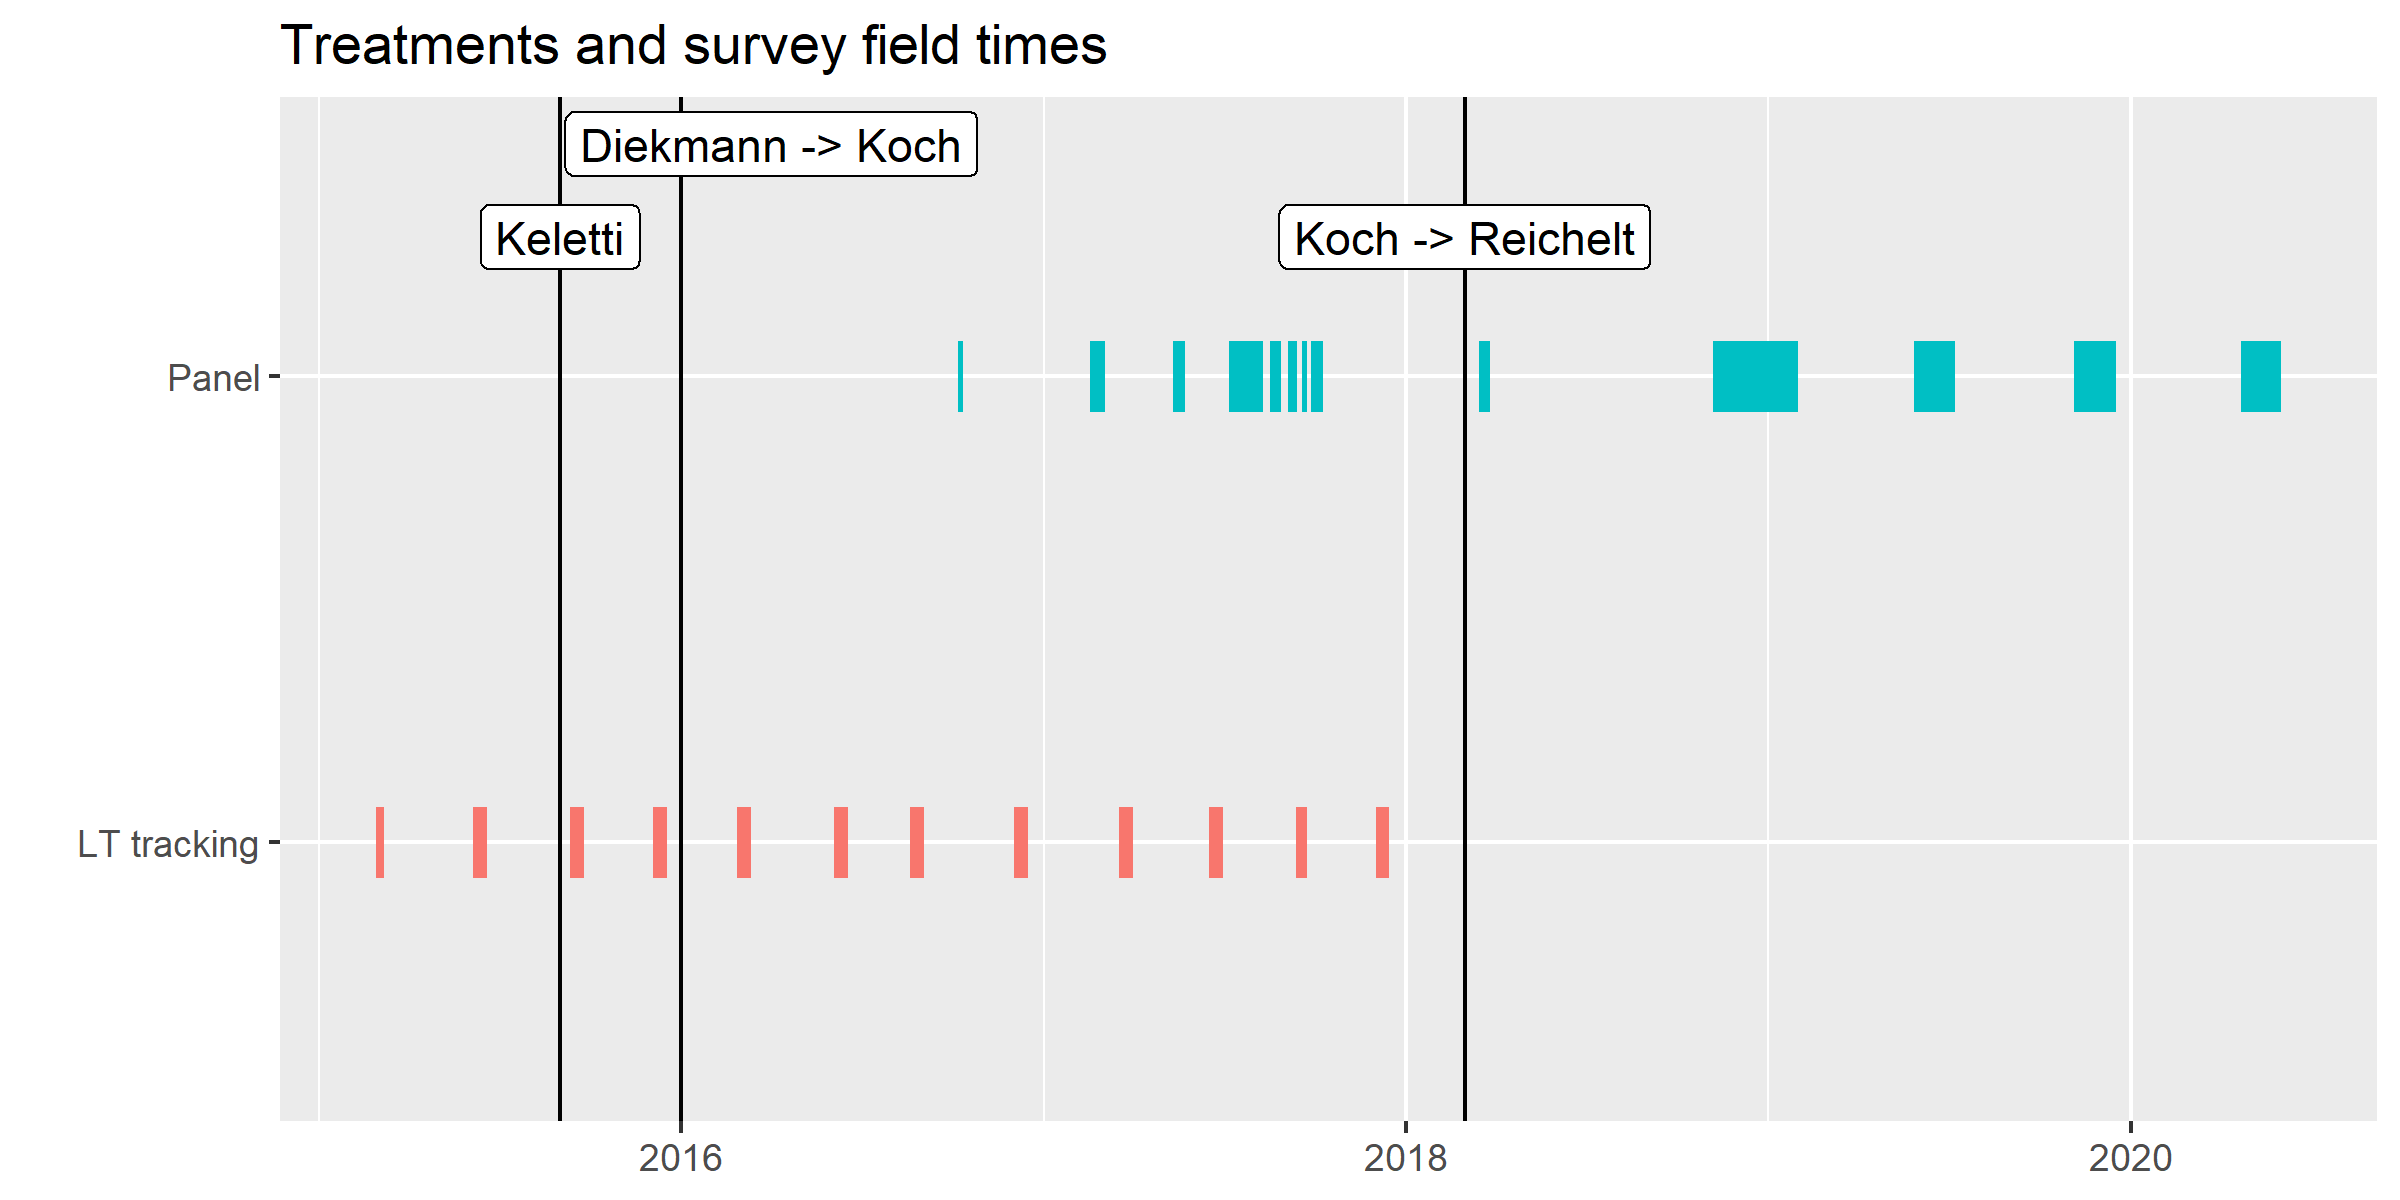
\includegraphics[width=\textwidth]{gles_treatments.png}
    \caption{Relative timing of possible shifts in migration framing and survey field times.}
    \label{fig:gles}
\end{figure}

Which treatment is viable will have to be decided based on an empirical comparison of the migration frames in \textit{Bild} to those in other newspapers. If the framing in \textit{Bild} diverges from a parallel trend with the framing of other newspapers, the treatment is viable. This will be measured by pre-selecting migration articles with supervised machine-learning classifiers, before using sentiment analysis to track the tone of migration coverage. 

After the selection of the viable treatment, a differences-in-differences design (DiD) will be estimated:

$$ y = \beta_1 * T + \beta_2 * B + \beta_3 * T * B $$

Where $y$ is the dependent (migration association or attitude), $T$ indicates the survey took place after the treatment/shift in migration framing, and $B$ indicates whether the respondent is a \textit{Bild}-reader. This means that the average of the dependent variable among \textit{Bild}-readers following the treatment is compared to non-\textit{Bild}-readers, both before and after the treatment, and \textit{Bild}-readers before treatment. $\beta_3$ - the quantity of interest - is then equal to the difference-in-differences, meaning the change in the dependent variable from before to after treatment, adjusted for the change among the control group (non-\textit{Bild} readers).

While the implementation is relatively straightforward for the migration attitude-variable using a five-point Likert scale, it is more complicated for the association of concepts with migration. Whether this can be measured is highly dependent on the number of responses discussing migration in the open answers to the most-important problem question. If possible, several surveys preceding and during the treatment (i.e. while the migration framing in \textit{Bild} differs from other newspapers) should be pooled to increase the number of respondents. 

To estimate the changing meaning of concepts in text, word embeddings have emerged as a state-of-the-art method. This method allows the numerical representation of semantic meaning in a high-dimensional vector-space. Those words with more similar meanings will occur closer together in the vector space, which allows the identification of changing meaning across corpora. However, these models require extensive training data (\cite{Rodman2019}). Recent work has tackled this problem by mapping embeddings into pre-trained, high-quality embedding spaces (\cite{Khodak2018}). This opens the possibility to quantitatively assess changing meaning in applications with few observations, such as open survey responses. Building on this work, \citeauthor{Rodriguez2020} have developed \textit{embedding regression}, which allows to express changing meanings as a function of covariates (\citeyear{Rodriguez2020}). Using the DiD to estimate these changes in meaning, it will be possible to understand how \textit{Bild}-readers understanding of migration changed following the treatment, compared to changes in the control group.

This will be compared to the outputs of the embedding regression for DiD with newspaper data, comparing migration framing in the \textit{Bild} before and after treatment to other newspapers before and after treatment. If the changes in the definition of migration indicated by the DiD are similar in the newspaper data and the survey responses, this constitutes strong evidence for a direct transmission of news frames into the issue definitions of consumers of these news.

% \textbf{[AV:  You should add info on who the part of people who actually write a lot are. Are they representative of BILD readers? Reichelt: Move from online editor to main editor? Does she have no influence on frames already? Do you have data on how ppl consume media?]}

\end{document}
